\documentclass[conference]{IEEEtran}

\usepackage[T1]{fontenc}
\usepackage[utf8]{inputenc}
\usepackage{cite}
\usepackage{amsmath,amssymb}
\usepackage{graphicx}
\usepackage{booktabs}
\usepackage{balance}
\usepackage{microtype}
\usepackage{xcolor}
\usepackage{url}
\urlstyle{same}

% Generated by Vibe Paper.
% Agents should read paper/context/project_snapshot.md before drafting.

\title{__PAPER_TITLE__}

\author{
\IEEEauthorblockN{__AUTHOR_NAME__}
\IEEEauthorblockA{
__AFFILIATION__\\
__EMAIL__
}
}

\begin{document}
\maketitle

\begin{abstract}
This template demonstrates a local-first workflow for writing English academic papers inside a real experiment repository. The goal is not to provide a final research manuscript, but to provide a stable paper workspace that can be attached to code, configs, logs, and exported metrics. The repository includes a reproducible build path, local preview support, reference management support, and a lightweight example figure so that users can start from a working baseline rather than from an empty directory.
\end{abstract}

\begin{IEEEkeywords}
LaTeX, academic writing, local workflow, paper workspace, agent-native editing
\end{IEEEkeywords}

\section{Introduction}
Many paper-writing workflows break down not because of research quality, but because the writing environment is brittle. A practical workflow should allow the author to edit a real LaTeX project, compile locally, manage references explicitly, and collaborate with AI tools without losing control of the source files. This template is intended to support that style of work inside a real experiment repository.

The example in this repository keeps the paper, figures, references, scripts, and build outputs in one project, while preserving the wider experiment folder as the evidence source. The structure also works well with AI-assisted editing because the model can modify the actual LaTeX source rather than operating on detached text fragments. For general background on LaTeX-based document preparation, see \cite{lamport1994latex}.

\section{Local Workflow}
The recommended workflow is straightforward. The author edits \texttt{main.tex}, stores references in \texttt{references/references.bib}, keeps generated figures in \texttt{figures/}, and compiles the paper through \texttt{build\_paper.bat}. The build path uses a temporary directory for compilation and then writes both a formal output PDF and a preview-safe copy. This approach is especially useful on Windows, where local preview can occasionally open a half-written PDF.

\begin{figure}[t]
\centering
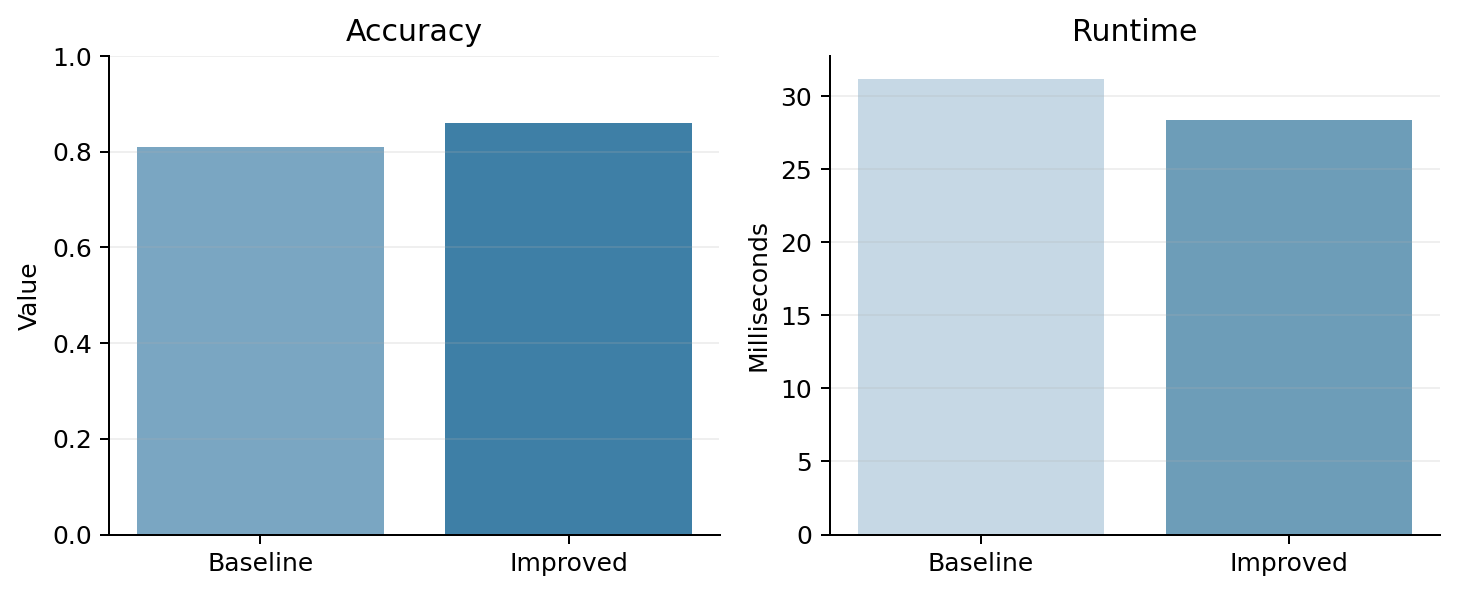
\includegraphics[width=\columnwidth]{figures/demo_metrics.png}
\caption{Example figure generated by the included Python script. The purpose of this figure is only to verify that the repository supports a paper-friendly workflow with scripts, figures, and local compilation.}
\label{fig:demo}
\end{figure}

\section{Example Table and Equation}
Table~\ref{tab:demo} shows a minimal result table. Equation~\eqref{eq:demo} is included to verify that the basic math setup is available.

\begin{table}[t]
\caption{Example result table}
\label{tab:demo}
\centering
\begin{tabular}{lcc}
\toprule
Method & Accuracy & Runtime \\
\midrule
Baseline & 0.81 & 31.2 ms \\
Improved & 0.86 & 28.4 ms \\
\bottomrule
\end{tabular}
\end{table}

\begin{equation}
\label{eq:demo}
\mathrm{Score} = \frac{TP}{TP + FP + FN}
\end{equation}

The purpose of these components is simple: if a user can compile this template successfully, then the same workspace structure can be reused for a real paper with relatively little effort.

\section{Conclusion}
This repository is intended to serve as a practical starting point for local LaTeX-based academic writing inside experiment projects. It provides a stable paper layout, a reproducible build path, local preview support, and an example that compiles immediately. Users can either edit the included sample or create a new paper workspace with the provided initialization script.

\balance
\bibliographystyle{IEEEtran}
\bibliography{references/references}

\end{document}
